\documentclass[10pt,a4paper,twoside,onecolumn]{article}

% Use UTF-8 for plain tex files
\usepackage[utf8]{inputenc}

% Advanced math support
\usepackage{amsmath}

% Huge list of math symbols
\usepackage{MnSymbol}

% Set the margin from the page side
\usepackage[margin=3cm]{geometry}

% Support for internal links
\usepackage{hyperref}
\hypersetup{
    colorlinks=true,
    linkcolor=black,
    citecolor=black,
    filecolor=black,
    urlcolor=black,
}

% Leave out page numbers on empty pages
\let\origdoublepage\cleardoublepage
\renewcommand{\cleardoublepage}{%
  \clearpage
  {\pagestyle{empty}\origdoublepage}%
}

% Don't indent paragrpahs, instead separate them
\usepackage{parskip}
\setlength{\parskip}{5mm plus2mm minus3mm}
\setlength{\parindent}{0cm}

% Use alternative font (see http://www.tug.dk/FontCatalogue/ for alternatives)
\usepackage{cmbright}
\renewcommand*\familydefault{\sfdefault} % Set the default font to be sans-serif
\usepackage[T1]{fontenc}

% Set line height multiplicity
\linespread{1.05}

% Allow URL typesetting
\usepackage{url}

% Customize captions appearances 
\usepackage[margin=1cm]{caption}
\DeclareCaptionFormat{listing}{{\em #1#2#3}}
\captionsetup{
	format=listing,
	font={small},
}

% Enable advanced style specifications for the basic listing environments
% (enumerate, itemize, description)
\usepackage{enumitem}

% Customize headers and footers
\usepackage{fancyhdr}

% Includegraphics support
\usepackage{graphicx}

% Allows to change text color
\usepackage[usenames,dvipsnames,table<D-+>]{xcolor}

% Assign the LastPage label to the last page
\usepackage{lastpage}

% Enable the creation of appendices
\usepackage{appendix}

% Support for lists
\usepackage{etoolbox}
\usepackage{fp}

% Advanced templating support
\newcommand{\settitle}[2]{%
	\title{#1 -- #2}
	\def\doctitle{#1}
	\def\subtitle{#2}
}
\newcounter{mseaindex}
\newcounter{mseacount}
\newcommand{\addauthor}[1]{%
	\listadd{\authors}{#1}
	\stepcounter{mseacount}
}
\newcommand{\fmtauthor}[1]{#1}
\newcommand{\lineslist}[1]{#1\\}
\newcommand{\authorlines}{%
	\setcounter{mseaindex}{0}%
	\FPdiv{\limit}{\arabic{mseacount}}{2}%
	\FPround{\limit}{\limit}{0}%
	\renewcommand*{\do}[1]{%
		\ifnumequal{\value{mseaindex}}{0}{}{\ifnumequal{\value{mseaindex}}{\limit}{}{, }}%
		\ifnumequal{\value{mseaindex}}{\limit}{\\[0.7mm]\fmtauthor{##1}}{\fmtauthor{##1}}%
		\stepcounter{mseaindex}%
	}%
	\dolistloop{\authors}%
}

% Set layout lenghts
\setlength{\headheight}{8mm}
\setlength{\footskip}{1.5cm}
\addtolength{\textheight}{-.5cm}

% Set titles whitespace
\usepackage{titlesec}
\titlespacing{\section}{0mm}{8mm}{1mm}
\titlespacing{\subsection}{0mm}{3mm}{-2mm}
\titlespacing{\subsubsection}{0mm}{2mm}{-1mm}

% Enable code listings and set default options
\usepackage{listings}
\usepackage{courier} % Use Adobe Courier instead of Computer Modern Typewriter
                     % for monospaced text
\lstloadlanguages{python,bash,sh,xml}
\lstset{
	language=python,
	basicstyle=\footnotesize\ttfamily,
	stringstyle=\color{OliveGreen},
	numbers=left,
	numberstyle=\color{gray}\tiny,
	commentstyle=\color{magenta},
	keywordstyle=\color{MidnightBlue}\bfseries,
	frame=bt,
	rulecolor=\color{lightgray},
	numbersep=7pt,
	escapechar=!,
	extendedchars=true,
	captionpos=t,
	breaklines=true,
	showspaces=false,
	showtabs=false,
	tabsize=4, 
	xleftmargin=20pt,
	framexleftmargin=20pt,
	framexrightmargin=0pt,
	framexbottommargin=0pt,
	showstringspaces=false,
}

% Limit the TOC dept to sections and subsections
\setcounter{tocdepth}{2}

\usepackage{multirow} % Enable columns spawning multiple rows
\usepackage{tabularx}
\usepackage{booktabs} % Provides {top|middle|bottom}rule
\usepackage{longtable} % Support for tables spawning multiple pages,
                       % captions and footnotes.
                       % Does not work in multicolumn environments
% Define new tabularx column types:
%  - R: streteched right aligned
%  - C: stretched centered
\newcolumntype{R}{>{\raggedleft\arraybackslash}X}%
\newcolumntype{C}{>{\centering\arraybackslash}X}%
\renewcommand{\arraystretch}{1.3} % Set row height multiplicator
\usepackage{threeparttable} % Manual footnotes counter

% Provide support for (indented) unnumbered chapter and section titles
\usepackage{tocloft}
\newcommand{\uchapter}[1]{
	\chapter*{#1}
	\addcontentsline{toc}{chapter}{\hspace{\cftchapnumwidth}#1}
}
\newcommand{\usection}[1]{
	\section*{#1}
	\addcontentsline{toc}{section}{\hspace{\cftsecnumwidth}#1}
}

% Color definitions
\definecolor{highlightyellow}{RGB}{255,255,140}
\definecolor{mselogogray}{RGB}{96,101,109} % Color definition for the MSE logo

% Enable highlighting using \HighlightFrom and \HighlightTo
\usepackage{classes/highlighter}
\tikzset{highlighter/.style = {highlightyellow, line width = \baselineskip*.75}}
 


\settitle{Lab. 04 -- Network scan}{Certified IT Security}
\addauthor{Julien Oberson}
\addauthor{Jonathan Stoppani}

\pagestyle{fancy}
\fancyhf{}
\renewcommand{\headrulewidth}{0pt}
\renewcommand{\footrulewidth}{0.6pt}

\fancyhead[LE]{%
	\raisebox{-0.15mm}{%
		
\includegraphics[height=6.3mm]{images/logo_mse_small}
		\hspace{5mm}\color{mselogogray}\rule[0mm]{0.5pt}{6mm}\hspace{4mm}}
	\begin{minipage}[b]{0.5\linewidth}
		\textcolor{mselogogray}{\uppercase{\scriptsize
			Certified IT Security\\[-1mm]
			Lab. 01 -- Port Scan}}
	\end{minipage}%
}

\fancyhead[RO]{%
	\begin{minipage}[b]{0.5\linewidth}
	\begin{flushright}
		\textcolor{mselogogray}{\uppercase{\scriptsize
			Julien Oberson\\[-1mm]
			Jonathan Stoppani}}
	\end{flushright}
	\end{minipage}
	\raisebox{-0.15mm}{%
		\hspace{4mm}\color{mselogogray}\rule[0mm]{0.5pt}{6mm}\hspace{5mm}
		
\includegraphics[height=6.3mm]{images/logo_mse_small}%
	}%
}

\fancyfoot[R]{\scriptsize\thepage\ of \pageref{LastPage}}
\fancyfoot[L]{\scriptsize\today}

\fancypagestyle{plain}{%
	\fancyhf{}
	\renewcommand{\footrulewidth}{0.6pt}
	\fancyfoot[R]{\scriptsize\thepage\ of \pageref{LastPage}}
	\fancyfoot[L]{\scriptsize\today}
}



\begin{document}

\title{Certified IT Secuirty\\  Lab. 01 -- Port scan}
\author{Julien Oberson \and Jonathan Stoppani}

\begin{titlepage}
\thispagestyle{empty}

\vspace*{10mm}

\includegraphics{images/logo_mse}
\vspace{5mm}

\hrule
\vspace{0.2mm}
{\Large Certified IT Security}\\[2mm]
{\Huge Lab. 01 -- Port scan}\\[1mm]
\hrule

\begin{minipage}[t]{0.5\textwidth}
    \begin{flushleft}
        Julien \textsc{Oberson}\\
        Jonathan \textsc{Stoppani}
    \end{flushleft}
\end{minipage}
\begin{minipage}[t]{0.495\textwidth}
	\begin{flushright}
        \today
	\end{flushright}
\end{minipage}

\vfill

\tableofcontents

\end{titlepage}


\cleardoublepage
\setcounter{page}{1}

\section{Introduction}

The goal of this laboratory session is to scan a given target (in this case, the scope is a local network segment) and find its operational security, controls and limitations as defined by the OSSTMM.

In our case, the scope are all the hosts on the local network segment \texttt{160.98.20.46-66} and the attack vector is from any machine inside the room \texttt{C0022} (Inside Network).

%******************************************************************************%
%******************************************************************************%

\section{Visibility}

The OSSTMM defines the term \textit{Visibility} as \textit{``the number of targets in the scope''}. In order to get the most precise view possible of the system, we execute an ARP scan using \texttt{nmap}. The results of the \texttt{sudo nmap -sP -PR 160.98.20.46-66} command are illustrated in the \autoref{lst:arp-scan}.

\lstset{label=lst:arp-scan,numbers=none,language=,caption=\texttt{nmap} ARP scan results}
\begin{lstlisting}
Starting Nmap 5.21 ( http://nmap.org ) at 2012-03-19 11:48 CET
Nmap scan report for c0022-1.tic.eia-fr.ch (160.98.20.46)
Host is up (0.00050s latency).
MAC Address: 00:19:D1:01:4C:A8 (Intel)
Nmap scan report for c0022-3.tic.eia-fr.ch (160.98.20.48)
Host is up (0.00053s latency).
MAC Address: 00:19:D1:25:E3:DB (Intel)
Nmap scan report for c0022-4.tic.eia-fr.ch (160.98.20.49)
Host is up (0.00054s latency).
MAC Address: 00:19:D1:25:E2:8F (Intel)
Nmap scan report for c0022-5.tic.eia-fr.ch (160.98.20.50)
Host is up (0.00055s latency).
MAC Address: 00:19:D1:25:E3:25 (Intel)
Nmap scan report for c0022-7.tic.eia-fr.ch (160.98.20.52)
Host is up (0.00052s latency).
MAC Address: 00:19:D1:25:E3:05 (Intel)
Nmap scan report for c0022-8.tic.eia-fr.ch (160.98.20.53)
Host is up (0.00053s latency).
MAC Address: 00:19:D1:25:E3:E1 (Intel)
Nmap scan report for c0022-10.tic.eia-fr.ch (160.98.20.55)
Host is up (0.00051s latency).
MAC Address: 00:19:D1:25:E3:F0 (Intel)
Nmap scan report for c0022-15.tic.eia-fr.ch (160.98.20.60)
Host is up (0.00052s latency).
MAC Address: 00:19:D1:25:E4:7F (Intel)
Nmap scan report for c0022-20.tic.eia-fr.ch (160.98.20.65)
Host is up (0.00051s latency).
MAC Address: 00:19:D1:25:E3:E9 (Intel)
Nmap done: !\HighlightFrom!21 IP addresses (9 hosts up)!\HighlightTo! scanned in 0.27 seconds
\end{lstlisting}

As shown in the command output, 9 hosts where found to be up and accessible over the local network.

%******************************************************************************%
%******************************************************************************%

\section{Access}

\textit{Access} is defined as \textit{``the number of unique interacton points, regardless of how many different ways this interaction point can be probed''}. In our specific case, this is the number of open TCP or UDP ports on each host.

\texttt{nmap} makes it easy to scan different hosts at once by defining an IP address range (using the same syntax as for the previous section). The commands used in this case are the following: \texttt{sudo nmap -sU 160.98.20.46-66} and \texttt{sudo nmap -sV -PN 160.98.20.46-66} (for UDP and TCP, respectively).

This chapter and the rest of this document are based on these scan results. You can find the detailed output in the appendices \ref{sec:tcp-scan} (for TCP) and \ref{sec:udp-scan} (for UDP), while the Table~\vref{tab:report} resumes the results along with their interpretation.

\begin{table}[p]
	\begin{threeparttable}
		\setlength{\tabcolsep}{5.8pt}
		\small\begin{tabularx}{\textwidth}{ R | c | c c c | c c c c c | c c c c c | c c c c c }
			\toprule

			% Headers
			\multirow{2}{*}{IP address} &
			\multirow{2}{*}{Up} &
			\multicolumn{3}{c|}{Open ports\tnote{1}} &
			\multicolumn{5}{c|}{Controls Class A\tnote{1}} &
			\multicolumn{5}{c|}{Controls Class B\tnote{1}} &
			\multicolumn{5}{c}{Limitations\tnote{1}} \\
			\cline{3-20}
			& & \hspace{-1mm}{\fontsize{6}{12} \selectfont TCP}\hspace{-1mm} & \hspace{-1mm}{\fontsize{6}{1}\selectfont UDP}\hspace{-1mm} & $\sum$ & A & I & S & C & R & N & C & P & I & A & V & W & C & E & A\\
			\hline

			% Contents
			160.98.20.46 & $\checkmark$ & 6 & 1 & 7 & 2 & - & - & - & - & 2 & 1 & 1 & 1 & 1 & - & 4 & - & 4 & - \\
			160.98.20.47 & - & - & - & - & - & - & - & - & - & - & - & - & - & - & - & - & - & - & - \\
			160.98.20.48 & $\checkmark$ & 3 & 3 & 6 & 2 & - & - & - & - & 1 & 1 & 1 & 1 & - & - & 2 & - & 2 & - \\
			160.98.20.49 & $\checkmark$ & 1 & - & 1 & 1 & - & - & - & - & 1 & 1 & 1 & 1 & - & - & 2 & - & 1 & - \\
			160.98.20.50 & $\checkmark$ & 1 & - & 1 & 1 & - & - & - & - & 1 & 1 & 1 & 1 & - & - & 2 & - & 1 & - \\
			160.98.20.51 & - & - & - & - & - & - & - & - & - & - & - & - & - & - & - & - & - & - & - \\
			160.98.20.52 & $\checkmark$ & 1 & - & 1 & 1 & - & - & - & - & 1 & 1 & 1 & 1 & - & - & 2 & - & 1 & - \\
			160.98.20.53 & - & - & - & - & - & - & - & - & - & - & - & - & - & - & - & - & - & - & - \\
			160.98.20.54 & - & - & - & - & - & - & - & - & - & - & - & - & - & - & - & - & - & - & - \\
			160.98.20.55 & $\checkmark$ & 1 & - & 1 & 1 & - & - & - & - & 1 & 1 & 1 & 1 & - & - & 2 & - & 1 & - \\
			160.98.20.56 & - & - & - & - & - & - & - & - & - & - & - & - & - & - & - & - & - & - & - \\
			160.98.20.57 & - & - & - & - & - & - & - & - & - & - & - & - & - & - & - & - & - & - & - \\
			160.98.20.58 & - & - & - & - & - & - & - & - & - & - & - & - & - & - & - & - & - & - & - \\
			160.98.20.59 & - & - & - & - & - & - & - & - & - & - & - & - & - & - & - & - & - & - & - \\
			160.98.20.60 & $\checkmark$ & 1 & - & 1 & 1 & - & - & - & - & 1 & 1 & 1 & 1 & - & - & 2 & - & 1 & - \\
			160.98.20.61 & - & - & - & - & - & - & - & - & - & - & - & - & - & - & - & - & - & - & - \\
			160.98.20.62 & - & - & - & - & - & - & - & - & - & - & - & - & - & - & - & - & - & - & - \\
			160.98.20.63 & - & - & - & - & - & - & - & - & - & - & - & - & - & - & - & - & - & - & - \\
			160.98.20.64 & - & - & - & - & - & - & - & - & - & - & - & - & - & - & - & - & - & - & - \\
			160.98.20.65 & $\checkmark$ & 1 & - & 1 & 1 & - & - & - & - & 1 & 1 & 1 & 1 & - & - & 2 & - & 1 & - \\
			160.98.20.66 & - & - & - & - & - & - & - & - & - & - & - & - & - & - & - & - & - & - & - \\
			\hline

			\raggedleft Totals & 8 & 15 & 7 & 22 & 10 & 0 & 0 & 0 & 0 & 9 & 8 & 8 & 8 & 1 & 0 & 18 & 0 & 12 & 0\\

			\bottomrule
		\end{tabularx}

		\begin{tablenotes}
		\item [1] See \autoref{tab:legend} for the meaning of the headers.
		\end{tablenotes}

		\caption{Summary of open ports, service information as detected by \texttt{nmap} and processes found by locally inspecting the target.}
		\label{tab:report}
	\end{threeparttable}
\end{table}

\begin{table}[p]
	\centering
	\subfloat[tab:leg2][Class A Controls]{
		\footnotesize\begin{tabularx}{0.3\textwidth}{ c | X }
			\toprule
			A & Authentication\\
			I & Indemnification\\
			S & Resistance\\
			C & Subjugation\\
			R & Continuity\\
			\bottomrule
		\end{tabularx}
	}
	\quad
	\subfloat[tab:leg2][Class B Controls]{
		\footnotesize\begin{tabularx}{0.3\textwidth}{ c | X }
			\toprule
			N & Non-Repudiation\\
			C & Confidentiality\\
			P & Privacy\\
			I & Integrity\\
			A & Alarm\\
			\bottomrule
		\end{tabularx}
	}
	\quad
	\subfloat[tab:leg2][Limitations]{
		\footnotesize\begin{tabularx}{0.3\textwidth}{ c | X }
			\toprule
			V & Vulnerabilities \\
			W & Weaknesses \\
			C & Concerns \\
			E & Exposures \\
			A & Anomalies \\
			\bottomrule
		\end{tabularx}
	}
	\caption{Legends for the column groups of the \autoref{tab:report}}
	\label{tab:legend}
\end{table}


%******************************************************************************%
%******************************************************************************%

\section{Trust}

Trust is the determination of trust relationships between a target and another entity (which can be a target too). A trust relationship exists wherever the target accepts interaction freely and without credentials. In this scope, trust is not relevant, so we won't consider it here.

%******************************************************************************%
%******************************************************************************%

\section{Class A -- Interactive Controls}

In this chapter, we explain how the values of the different class A controls (resumed in the \autoref{tab:report}) are obtained.

\subsection{Autentication}
% If you want a smaller bullet:
%\newcommand{\sbt}{\,\begin{picture}(-1,1)(-1,-3)\circle*{3}\end{picture}\ }
%\renewcommand{\labelitemi}{$\sbt$}
\begin{itemize}
	\setlength{\itemsep}{-3mm}
	\item SSH services on all hosts ask for a password;
	\item Telnet service ask for a password;
	\item VMware SSL/Auth ask for a password;
	\item VMware Auth ask for a password.
\end{itemize}

\subsection{Indemnification}

There are no idenmnification measures observed on the discovered services.

\subsection{Resilience}

These hosts are workstation and not servers. Resilience measures are not implemented in the discovered applications. This information is known because we simulate a test in which hosts in the scope are known (Tandem test).

\subsection{Subjugation}

There are no subjugation measures observed on the discovered services.

\subsection{Continuity}

Smiliarly as seen before, these hosts are workstation and not servers and continuity measures are thus not implemented in the discovered applications.

%******************************************************************************%
%******************************************************************************%

\section{Class B -- Process Controls}

In this chapter, we explain how the values of the different class B controls (presented in \autoref{tab:report}) are obtained.

\subsection{Non-repudiation}

\begin{itemize}
	\setlength{\itemsep}{-3mm}
	\item SSH login attempts (success \& fail) are logged through the system logger;
	\item VMware SSL/Auth login attempts (success \& fail) are logged in the VMware logs;
	\item VMware Auth login attempts (success \& fail) are logged in the VMware logs.
\end{itemize}

\subsection{Confidentility, authenticity \& integrity}

\begin{itemize}
	\setlength{\itemsep}{-3mm}
	\item SSH communications are encrypted, authenticated and integrity-protected;
	\item VMware SSL/Auth communications are encrypted, authenticated and integrity-protected.
\end{itemize}

\subsection{Alarm}

Linux hosts are workstations without any antivirus nor IDS. The host at \texttt{160.98.20.46} is a windows host with an antivirus and is thus able to fire an alarm. This information is known because we simulate a test in which the hosts in the scope are known (Tandem test).

%******************************************************************************%
%******************************************************************************%

\section{Limitations}

\subsection{Exposures}

In this section, we report useless information exposed by the different scanned hosts.

\begin{itemize}
	\setlength{\itemsep}{-3mm}
	\item Microsoft Windows RPC exposes the used software;
	\item SSH server exposes running software and his version;
	\item VMware Authentification Deamon exposes his version;
	\item VMware Authentification Deamon with SSL exposes his version;
	\item Tenlet server exposes the used software;
	\item NAI EPO Agent exposes the used software and his version.
\end{itemize}

\subsection{Vulnerabilities}

No vulnerabilities were detected on the discovered services.

\subsection{Weaknesses}

\begin{itemize}
	\item The running OpenSSH server is at version 5.6. This version has two known vulnerabilties: \texttt{CVE-2010-4478} and \texttt{CVE-2010-4478}. These two vulnerabilities don't permit direct access to the machine can thus be classified as weaknesses and not as vunerabilities.
	\item The running version of the vmware-auth daemon has four known vulnerabilties: \texttt{CVE-2009-4811}, \texttt{CVE-2009-3707}, \texttt{CVE-2009-0177} and \texttt{CVE-2008-0967}. As before, the exploitation of these four vulnerabilities doesn't allow to directly access the machine and can thus be classified as weaknesses instead of vunerabilities.

\end{itemize}

\subsection{Concerns}

No concerns were observed on the discovered services.

\subsection{Anomalies}

No anomalies were encountered during the tests.

%******************************************************************************%
%******************************************************************************%

\appendix

\clearpage
\section{\texttt{nmap} TCP Scan Result}
\label{sec:tcp-scan}

\lstset{label=lst:tcp-scan,numbers=none,language=,caption=\texttt{nmap} TCP scan results}
\begin{lstlisting}
Starting Nmap 5.21 ( http://nmap.org ) at 2012-03-19 12:50 CET
Nmap scan report for c0022-1.tic.eia-fr.ch (160.98.20.46)
Host is up (0.00070s latency).
Not shown: 994 filtered ports
PORT     STATE SERVICE         VERSION
135/tcp  open  msrpc           Microsoft Windows RPC
139/tcp  open  netbios-ssn
445/tcp  open  netbios-ssn
902/tcp  open  ssl/vmware-auth VMware Authentication Daemon 1.10 (Uses VNC, SOAP)
912/tcp  open  vmware-auth     VMware Authentication Daemon 1.0 (Uses VNC, SOAP)
8081/tcp open  http            NAI EPO Agent framework (Agent ListenServer 1.0)
MAC Address: 00:19:D1:01:4C:A8 (Intel)
Service Info: OS: Windows

Nmap scan report for c0022-3.tic.eia-fr.ch (160.98.20.48)
Host is up (0.00044s latency).
Not shown: 997 closed ports
PORT    STATE SERVICE VERSION
22/tcp  open  ssh     OpenSSH 5.6 (protocol 2.0)
23/tcp  open  telnet  Linux telnetd
111/tcp open  rpcbind
MAC Address: 00:19:D1:25:E3:DB (Intel)
Service Info: OS: Linux

Nmap scan report for c0022-4.tic.eia-fr.ch (160.98.20.49)
Host is up (0.00053s latency).
Not shown: 999 filtered ports
PORT   STATE SERVICE VERSION
22/tcp open  ssh     OpenSSH 5.6 (protocol 2.0)
MAC Address: 00:19:D1:25:E2:8F (Intel)

Nmap scan report for c0022-5.tic.eia-fr.ch (160.98.20.50)
Host is up (0.00054s latency).
Not shown: 999 filtered ports
PORT   STATE SERVICE VERSION
22/tcp open  ssh     OpenSSH 5.6 (protocol 2.0)
MAC Address: 00:19:D1:25:E3:25 (Intel)

Nmap scan report for c0022-7.tic.eia-fr.ch (160.98.20.52)
Host is up (0.00055s latency).
Not shown: 999 filtered ports
PORT   STATE SERVICE VERSION
22/tcp open  ssh     OpenSSH 5.6 (protocol 2.0)
MAC Address: 00:19:D1:25:E3:05 (Intel)

Nmap scan report for c0022-10.tic.eia-fr.ch (160.98.20.55)
Host is up (0.00054s latency).
Not shown: 999 filtered ports
PORT   STATE SERVICE VERSION
22/tcp open  ssh     OpenSSH 5.6 (protocol 2.0)
MAC Address: 00:19:D1:25:E3:F0 (Intel)

Nmap scan report for c0022-15.tic.eia-fr.ch (160.98.20.60)
Host is up (0.00054s latency).
Not shown: 999 filtered ports
PORT   STATE SERVICE VERSION
22/tcp open  ssh     OpenSSH 5.6 (protocol 2.0)
MAC Address: 00:19:D1:25:E4:7F (Intel)

Nmap scan report for c0022-20.tic.eia-fr.ch (160.98.20.65)
Host is up (0.00054s latency).
Not shown: 999 filtered ports
PORT   STATE SERVICE VERSION
22/tcp open  ssh     OpenSSH 5.6 (protocol 2.0)
MAC Address: 00:19:D1:25:E3:E9 (Intel)

Service detection performed. Please report any incorrect results at http://nmap.org/submit/ .
Nmap done: 21 IP addresses (8 hosts up) scanned in 22.71 seconds
\end{lstlisting}

\clearpage
\section{\texttt{nmap} UDP Scan Results}
\label{sec:udp-scan}

\lstset{label=lst:udp-scan,numbers=none,language=,caption=\texttt{nmap} UDP scan results}
\begin{lstlisting}
Starting Nmap 5.21 ( http://nmap.org ) at 2012-03-19 13:07 CET
Nmap scan report for c0022-1.tic.eia-fr.ch (160.98.20.46)
Host is up (0.00072s latency).
Not shown: 999 open|filtered ports
PORT    STATE SERVICE
137/udp open  netbios-ns
MAC Address: 00:19:D1:01:4C:A8 (Intel)

Nmap scan report for c0022-3.tic.eia-fr.ch (160.98.20.48)
Host is up (0.00058s latency).
Not shown: 994 closed ports
PORT     STATE         SERVICE
68/udp   open|filtered dhcpc
111/udp  open          rpcbind
123/udp  open          ntp
631/udp  open|filtered ipp
643/udp  open|filtered unknown
5353/udp open          zeroconf
MAC Address: 00:19:D1:25:E3:DB (Intel)

Nmap scan report for c0022-4.tic.eia-fr.ch (160.98.20.49)
Host is up (0.00056s latency).
All 1000 scanned ports on c0022-4.tic.eia-fr.ch (160.98.20.49) are filtered
MAC Address: 00:19:D1:25:E2:8F (Intel)

Nmap scan report for c0022-5.tic.eia-fr.ch (160.98.20.50)
Host is up (0.00053s latency).
All 1000 scanned ports on c0022-5.tic.eia-fr.ch (160.98.20.50) are filtered
MAC Address: 00:19:D1:25:E3:25 (Intel)

Nmap scan report for c0022-7.tic.eia-fr.ch (160.98.20.52)
Host is up (0.00054s latency).
All 1000 scanned ports on c0022-7.tic.eia-fr.ch (160.98.20.52) are filtered
MAC Address: 00:19:D1:25:E3:05 (Intel)

Nmap scan report for c0022-10.tic.eia-fr.ch (160.98.20.55)
Host is up (0.00057s latency).
All 1000 scanned ports on c0022-10.tic.eia-fr.ch (160.98.20.55) are filtered
MAC Address: 00:19:D1:25:E3:F0 (Intel)

Nmap scan report for c0022-15.tic.eia-fr.ch (160.98.20.60)
Host is up (0.00057s latency).
All 1000 scanned ports on c0022-15.tic.eia-fr.ch (160.98.20.60) are filtered
MAC Address: 00:19:D1:25:E4:7F (Intel)

Nmap scan report for c0022-20.tic.eia-fr.ch (160.98.20.65)
Host is up (0.00054s latency).
All 1000 scanned ports on c0022-20.tic.eia-fr.ch (160.98.20.65) are filtered
MAC Address: 00:19:D1:25:E3:E9 (Intel)

Nmap done: 21 IP addresses (8 hosts up) scanned in 1086.60 seconds
\end{lstlisting}

\clearpage
\section{RAV calculation for \texttt{160.98.20.46}}
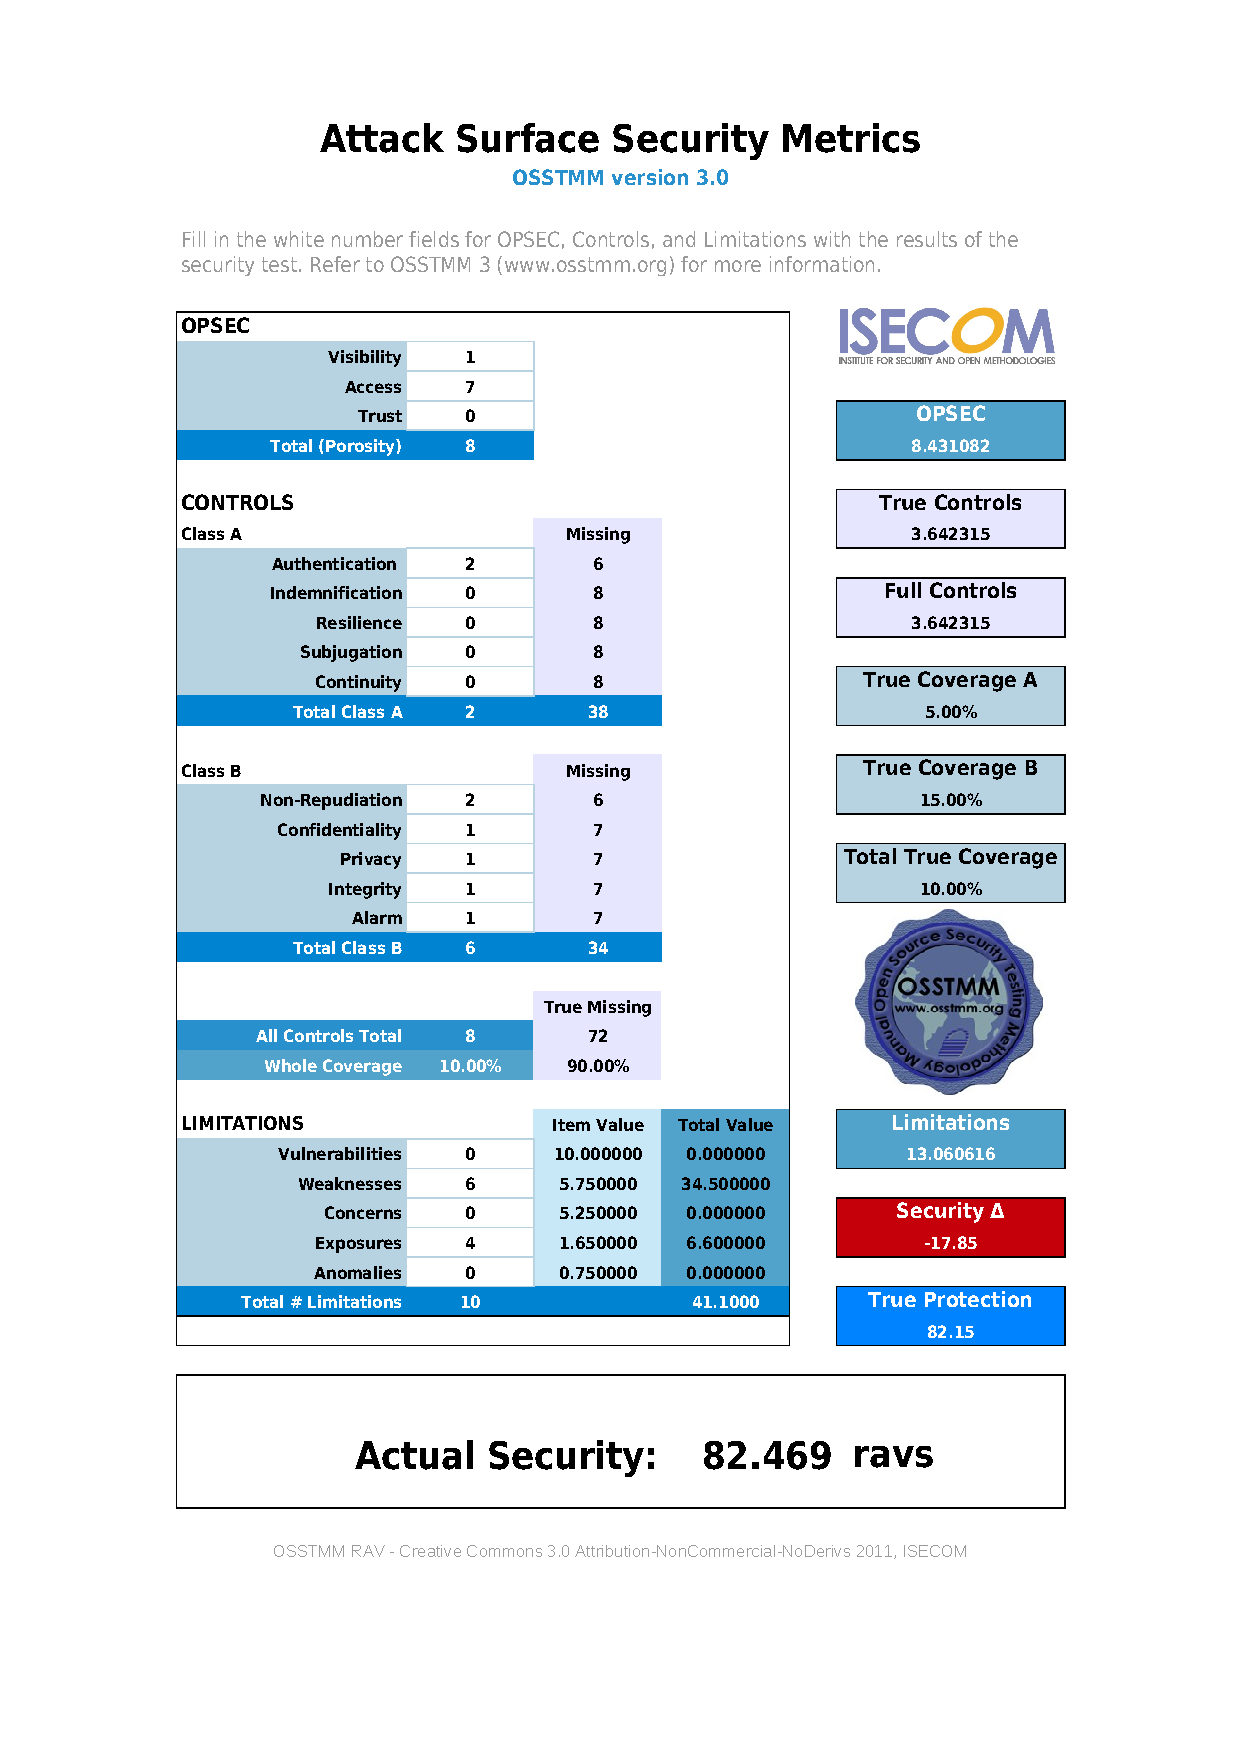
\includegraphics[width=\textwidth,trim=84pt 110pt 84pt 140pt,clip=true]{data/160982046.pdf}

\clearpage
\section{RAV calculation for the entire scope}
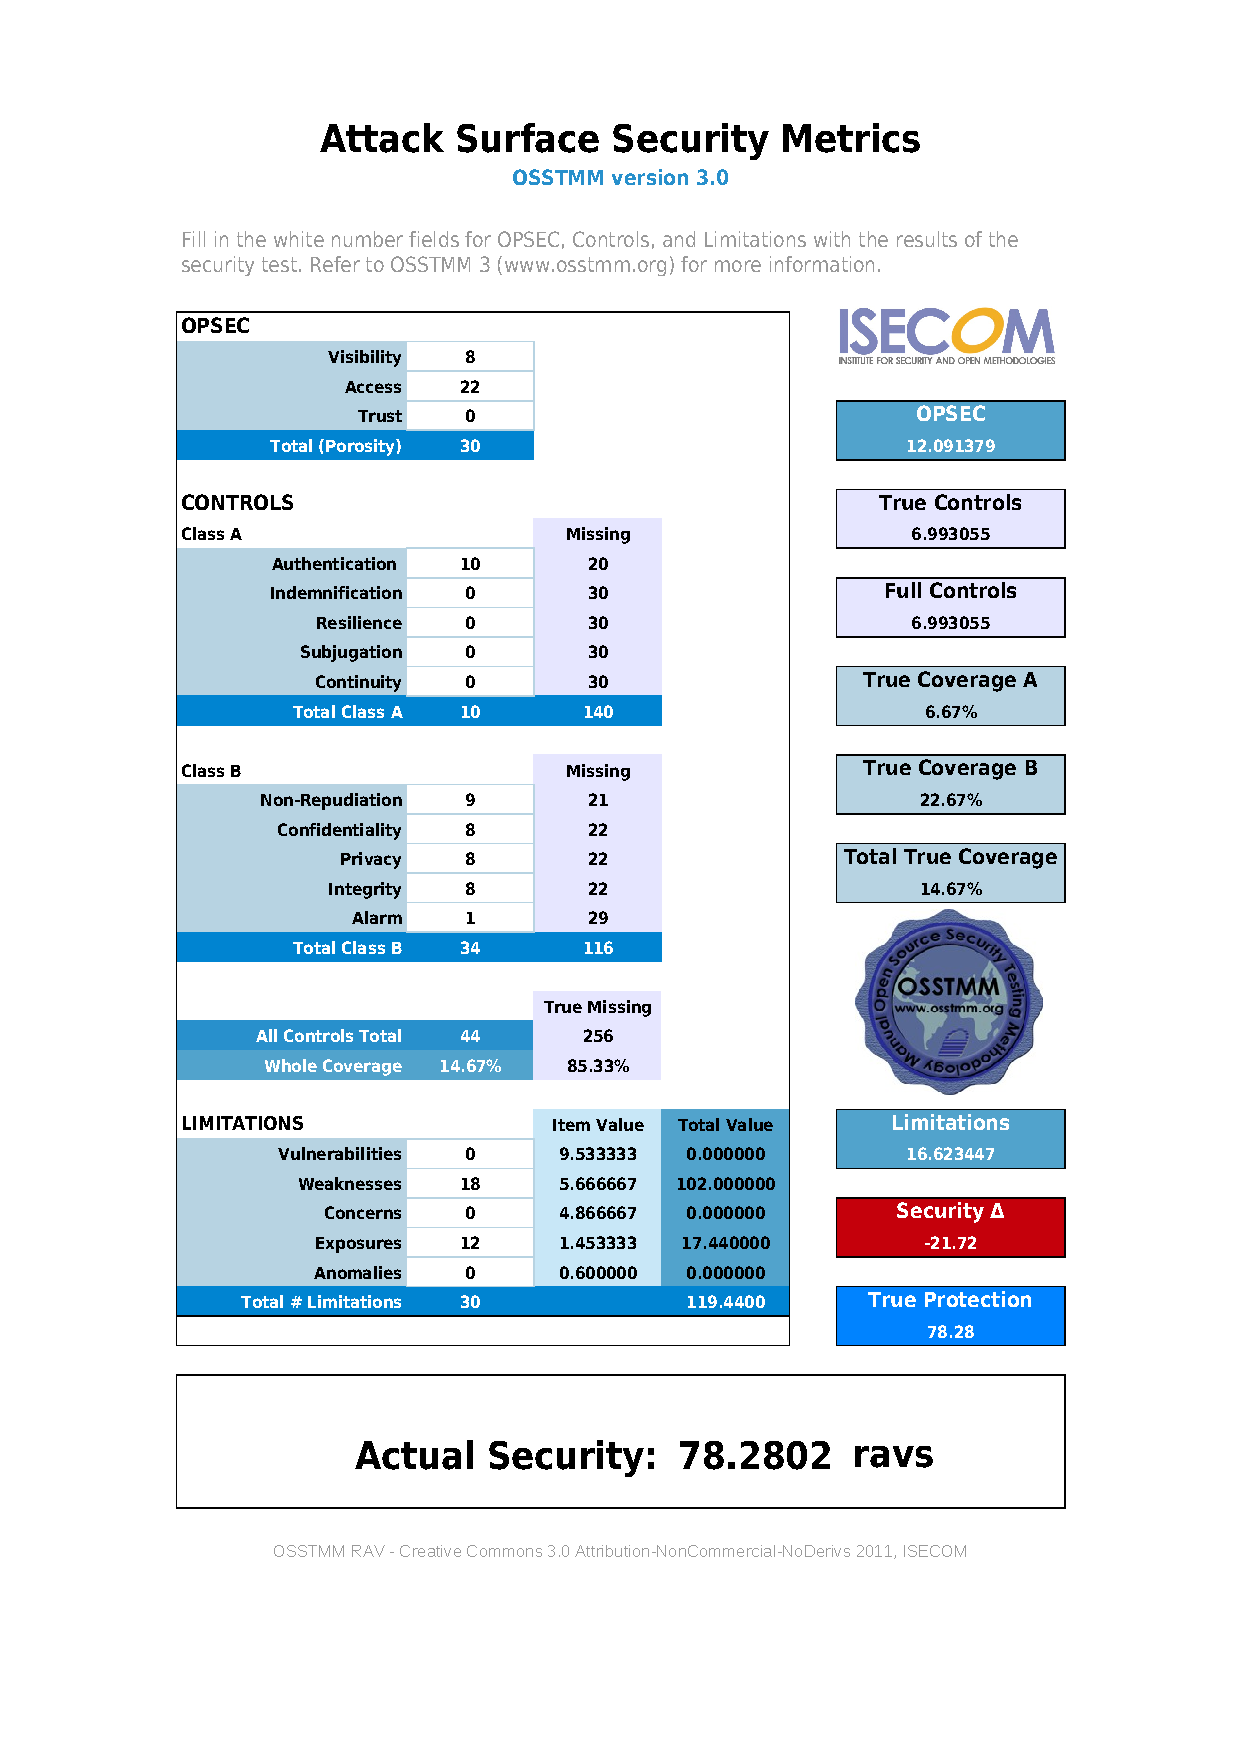
\includegraphics[width=\textwidth,trim=84pt 110pt 84pt 140pt,clip=true]{data/global.pdf}

\end{document}
